\documentclass{standalone}
\usepackage{tikz}
\usetikzlibrary{patterns, positioning}

\begin{document}
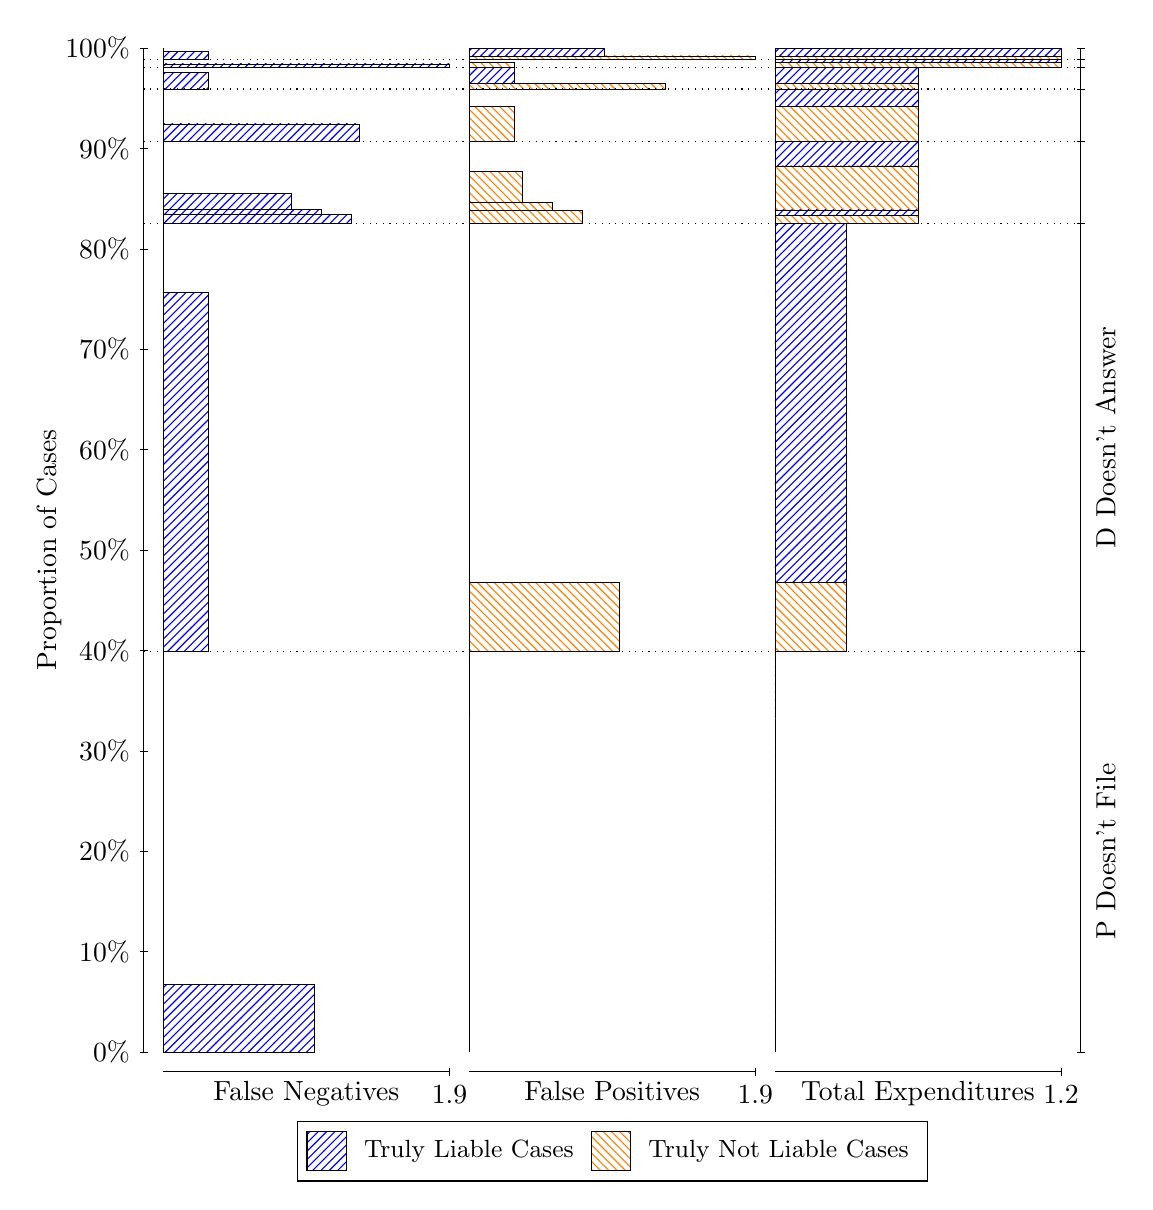
\begin{tikzpicture}
\draw[black, very thin] (1.5,1.75) -- (1.5,14.5);
\node[rotate=90, anchor=center] at (0.3, 8.125) {Proportion of Cases};
\draw[black, very thin] (1.45,1.75) -- (1.55,1.75);
\node[anchor=east] at (1.45, 1.75) {0\%};
\draw[black, very thin] (1.45,3.025) -- (1.55,3.025);
\node[anchor=east] at (1.45, 3.025) {10\%};
\draw[black, very thin] (1.45,4.3) -- (1.55,4.3);
\node[anchor=east] at (1.45, 4.3) {20\%};
\draw[black, very thin] (1.45,5.575) -- (1.55,5.575);
\node[anchor=east] at (1.45, 5.575) {30\%};
\draw[black, very thin] (1.45,6.85) -- (1.55,6.85);
\node[anchor=east] at (1.45, 6.85) {40\%};
\draw[black, very thin] (1.45,8.125) -- (1.55,8.125);
\node[anchor=east] at (1.45, 8.125) {50\%};
\draw[black, very thin] (1.45,9.4) -- (1.55,9.4);
\node[anchor=east] at (1.45, 9.4) {60\%};
\draw[black, very thin] (1.45,10.675) -- (1.55,10.675);
\node[anchor=east] at (1.45, 10.675) {70\%};
\draw[black, very thin] (1.45,11.95) -- (1.55,11.95);
\node[anchor=east] at (1.45, 11.95) {80\%};
\draw[black, very thin] (1.45,13.225) -- (1.55,13.225);
\node[anchor=east] at (1.45, 13.225) {90\%};
\draw[black, very thin] (1.45,14.5) -- (1.55,14.5);
\node[anchor=east] at (1.45, 14.5) {100\%};

\draw[black, very thin] (13.4,1.75) -- (13.4,14.5);
\draw[black, very thin] (13.35,1.75) -- (13.45,1.75);
\node[anchor=west] at (13.35, 1.75) {};
\draw[black, very thin] (13.35,6.8406) -- (13.45,6.8406);
\node[anchor=west] at (13.35, 6.8406) {};
\draw[black, very thin] (13.35,12.27) -- (13.45,12.27);
\node[anchor=west] at (13.35, 12.27) {};
\draw[black, very thin] (13.35,13.313) -- (13.45,13.313);
\node[anchor=west] at (13.35, 13.313) {};
\draw[black, very thin] (13.35,13.98) -- (13.45,13.98);
\node[anchor=west] at (13.35, 13.98) {};
\draw[black, very thin] (13.35,14.256) -- (13.45,14.256);
\node[anchor=west] at (13.35, 14.256) {};
\draw[black, very thin] (13.35,14.358) -- (13.45,14.358);
\node[anchor=west] at (13.35, 14.358) {};
\draw[black, very thin] (13.35,14.5) -- (13.45,14.5);
\node[anchor=west] at (13.35, 14.5) {};

\draw[black, very thin, pattern color=blue, pattern=north east lines] (1.75,1.75) rectangle (3.6623,2.6054);
\draw[black, very thin, pattern color=orange, pattern=north west lines] (1.75,2.6054) rectangle (1.75,6.8406);
\draw[black, very thin, pattern color=blue, pattern=north east lines] (1.75,6.8406) rectangle (2.3237,11.401);
\draw[black, very thin, pattern color=orange, pattern=north west lines] (1.75,11.401) rectangle (1.75,12.27);
\draw[black, very thin, pattern color=blue, pattern=north east lines] (1.75,12.27) rectangle (4.1404,12.383);
\draw[black, very thin, pattern color=blue, pattern=north east lines] (1.75,12.383) rectangle (3.7579,12.455);
\draw[black, very thin, pattern color=blue, pattern=north east lines] (1.75,12.455) rectangle (3.3754,12.653);
\draw[black, very thin, pattern color=orange, pattern=north west lines] (1.75,12.653) rectangle (1.75,13.313);
\draw[black, very thin, pattern color=blue, pattern=north east lines] (1.75,13.313) rectangle (4.236,13.538);
\draw[black, very thin, pattern color=orange, pattern=north west lines] (1.75,13.538) rectangle (1.75,13.98);
\draw[black, very thin, pattern color=blue, pattern=north east lines] (1.75,13.98) rectangle (2.3237,14.189);
\draw[black, very thin, pattern color=orange, pattern=north west lines] (1.75,14.189) rectangle (1.75,14.256);
\draw[black, very thin, pattern color=blue, pattern=north east lines] (1.75,14.256) rectangle (5.3833,14.299);
\draw[black, very thin, pattern color=orange, pattern=north west lines] (1.75,14.299) rectangle (1.75,14.358);
\draw[black, very thin, pattern color=blue, pattern=north east lines] (1.75,14.358) rectangle (2.3237,14.458);
\draw[black, very thin, pattern color=orange, pattern=north west lines] (1.75,14.458) rectangle (1.75,14.5);
\draw[black, very thin, pattern color=orange, pattern=north west lines] (5.6333,1.75) rectangle (5.6333,5.9852);
\draw[black, very thin, pattern color=blue, pattern=north east lines] (5.6333,5.9852) rectangle (5.6333,6.8406);
\draw[black, very thin, pattern color=orange, pattern=north west lines] (5.6333,6.8406) rectangle (7.5456,7.7095);
\draw[black, very thin, pattern color=blue, pattern=north east lines] (5.6333,7.7095) rectangle (5.6333,12.27);
\draw[black, very thin, pattern color=orange, pattern=north west lines] (5.6333,12.27) rectangle (7.0675,12.434);
\draw[black, very thin, pattern color=orange, pattern=north west lines] (5.6333,12.434) rectangle (6.6851,12.537);
\draw[black, very thin, pattern color=orange, pattern=north west lines] (5.6333,12.537) rectangle (6.3026,12.93);
\draw[black, very thin, pattern color=blue, pattern=north east lines] (5.6333,12.93) rectangle (5.6333,13.313);
\draw[black, very thin, pattern color=orange, pattern=north west lines] (5.6333,13.313) rectangle (6.207,13.755);
\draw[black, very thin, pattern color=blue, pattern=north east lines] (5.6333,13.755) rectangle (5.6333,13.98);
\draw[black, very thin, pattern color=orange, pattern=north west lines] (5.6333,13.98) rectangle (8.1193,14.048);
\draw[black, very thin, pattern color=blue, pattern=north east lines] (5.6333,14.048) rectangle (6.207,14.256);
\draw[black, very thin, pattern color=orange, pattern=north west lines] (5.6333,14.256) rectangle (6.207,14.315);
\draw[black, very thin, pattern color=blue, pattern=north east lines] (5.6333,14.315) rectangle (5.6333,14.358);
\draw[black, very thin, pattern color=orange, pattern=north west lines] (5.6333,14.358) rectangle (9.2667,14.4);
\draw[black, very thin, pattern color=blue, pattern=north east lines] (5.6333,14.4) rectangle (7.3544,14.5);
\draw[black, very thin, pattern color=orange, pattern=north west lines] (9.5167,1.75) rectangle (9.5167,5.9852);
\draw[black, very thin, pattern color=blue, pattern=north east lines] (9.5167,5.9852) rectangle (9.5167,6.8406);
\draw[black, very thin, pattern color=orange, pattern=north west lines] (9.5167,6.8406) rectangle (10.425,7.7095);
\draw[black, very thin, pattern color=blue, pattern=north east lines] (9.5167,7.7095) rectangle (10.425,12.27);
\draw[black, very thin, pattern color=orange, pattern=north west lines] (9.5167,12.27) rectangle (11.333,12.373);
\draw[black, very thin, pattern color=blue, pattern=north east lines] (9.5167,12.373) rectangle (11.333,12.445);
\draw[black, very thin, pattern color=orange, pattern=north west lines] (9.5167,12.445) rectangle (11.333,13.002);
\draw[black, very thin, pattern color=blue, pattern=north east lines] (9.5167,13.002) rectangle (11.333,13.313);
\draw[black, very thin, pattern color=orange, pattern=north west lines] (9.5167,13.313) rectangle (11.333,13.755);
\draw[black, very thin, pattern color=blue, pattern=north east lines] (9.5167,13.755) rectangle (11.333,13.98);
\draw[black, very thin, pattern color=orange, pattern=north west lines] (9.5167,13.98) rectangle (11.333,14.048);
\draw[black, very thin, pattern color=blue, pattern=north east lines] (9.5167,14.048) rectangle (11.333,14.256);
\draw[black, very thin, pattern color=orange, pattern=north west lines] (9.5167,14.256) rectangle (13.15,14.315);
\draw[black, very thin, pattern color=blue, pattern=north east lines] (9.5167,14.315) rectangle (13.15,14.358);
\draw[black, very thin, pattern color=orange, pattern=north west lines] (9.5167,14.358) rectangle (13.15,14.4);
\draw[black, very thin, pattern color=blue, pattern=north east lines] (9.5167,14.4) rectangle (13.15,14.5);
\draw[black, dotted] (1.5,6.8406) -- (13.4,6.8406);
\draw[black, dotted] (1.5,12.27) -- (13.4,12.27);
\draw[black, dotted] (1.5,13.313) -- (13.4,13.313);
\draw[black, dotted] (1.5,13.98) -- (13.4,13.98);
\draw[black, dotted] (1.5,14.256) -- (13.4,14.256);
\draw[black, dotted] (1.5,14.358) -- (13.4,14.358);
\draw[black, very thin] (1.75,1.5) -- (5.3833,1.5);
\node[anchor=north] at (3.5667, 1.5) {False Negatives};
\draw[black, very thin] (5.3833,1.45) -- (5.3833,1.55);
\node[anchor=north] at (5.3833, 1.45) {1.9};

\draw[black, very thin] (5.6333,1.5) -- (9.2667,1.5);
\node[anchor=north] at (7.45, 1.5) {False Positives};
\draw[black, very thin] (9.2667,1.45) -- (9.2667,1.55);
\node[anchor=north] at (9.2667, 1.45) {1.9};

\draw[black, very thin] (9.5167,1.5) -- (13.15,1.5);
\node[anchor=north] at (11.333, 1.5) {Total Expenditures};
\draw[black, very thin] (13.15,1.45) -- (13.15,1.55);
\node[anchor=north] at (13.15, 1.45) {1.2};

\node[black, centered, rotate=90] at (13.72, 4.2953) {P Doesn't File};
\node[black, centered, rotate=90] at (13.72, 9.5553) {D Doesn't Answer};






\draw (7.449999999999999,1.5) node[draw=none] (baseCoordinate) {};
\begin{scope}[align=center]
        \matrix[scale=0.5, draw=black, below=0.5cm of baseCoordinate, nodes={draw}, column sep=0.1cm]{
            \node[rectangle, draw, minimum width=0.5cm, minimum height=0.5cm, pattern=north east lines, pattern color=blue] {}; &
            \node[draw=none, font=\small] (B) {Truly Liable Cases}; &
            \node[rectangle, draw, minimum width=0.5cm, minimum height=0.5cm, pattern=north west lines, pattern color=orange] {}; &
            \node[draw=none, font=\small] (B) {Truly Not Liable Cases}; \\
            };
\end{scope}

\end{tikzpicture}
\end{document}